\documentclass{article}

\usepackage[scheme=plain]{ctex}

\usepackage{listings}
\usepackage{xcolor}
\usepackage{graphicx}
\usepackage{float}
\usepackage{subcaption}
\usepackage{fullpage}

\usepackage{amsfonts, amssymb, amsmath}
\usepackage{mathrsfs}

%\lstset{
%  basicstyle=\ttfamily, % Set font to a monospaced family
%  breaklines=true,      % Enable automatic line breaking
%  postbreak=\mbox{\textcolor{gray}{$\hookrightarrow$}\space}  
%}

\title{YouZhiSan User's Guide}
\date{2025}
\author{Qi Dawei}

\begin{document}

\maketitle

\section{Introduction}
YouZhiSan is a wrapper for the popular PyCrystalField\cite{scheiePyCrystalFieldSoftwareCalculation2021} program, designed to extend its capabilities to include excited states. This feature is essential for fitting data from optical spectroscopy.

It also bundles several other tools to create a complete, "out-of-the-box" solution. The goal is to make the process as simple as possible—allowing a user to fit a crystal field Hamiltonian with minimal setup, ideally just by pressing the "start" button.

Current Ion Support:
\begin{itemize}
\item Full Excited states: Nd3+, Dy3+, Pr3+, Er3+, Tm3+, Yb3+, Eu3+, Sm3+
\item Excited states with cubic symmetry: Tb3+
\item Ground states only: Ce3+, Pm3+, Ho3+
\end{itemize}
All physical quantities with the dimension of energy are expressed in units of meV
\section{Name}
YouZhiSan (oil-papered umbrella) is a traditional handicraft deeply rooted in Fuzhou culture. These umbrellas are celebrated for their graceful style, which combines beautiful symmetrical patterns and rich, vibrant colours.

This serves as a metaphor for crystal field theory, where the structure's symmetry dictates the splitting of energy levels that manifest as colourful spectroscopic peaks.
\section{Installation}
YouZhiSan is a script-based program, not a package you need to install. It’s compatible with any Python environment that has PyCrystalField properly configured. That said, we strongly recommend using Anaconda with Spyder for the smoothest workflow.

To install PyCrystalField, run the following command in your Anaconda Prompt (or any terminal where Anaconda is activated):

%\lstset{
%    basicstyle=\ttfamily,
%    breaklines=true
%}
\begin{lstlisting}[
    basicstyle=\ttfamily,
    breaklines=True
]
pip install git+https://github.com/asche1/PyCrystalField.git@master
\end{lstlisting}

For users who may experience difficulties accessing GitHub under certain network environments, you can try configuring Git to use a locally running HTTP and HTTPS proxy. Alternatively, you could ask a friend with unrestricted access to download the entire PyCrystalField repository as a ZIP file. They can then send the file to you, and you can install it locally using pip.

\begin{figure}[H]

    \begin{subfigure}{0.45\textwidth}

        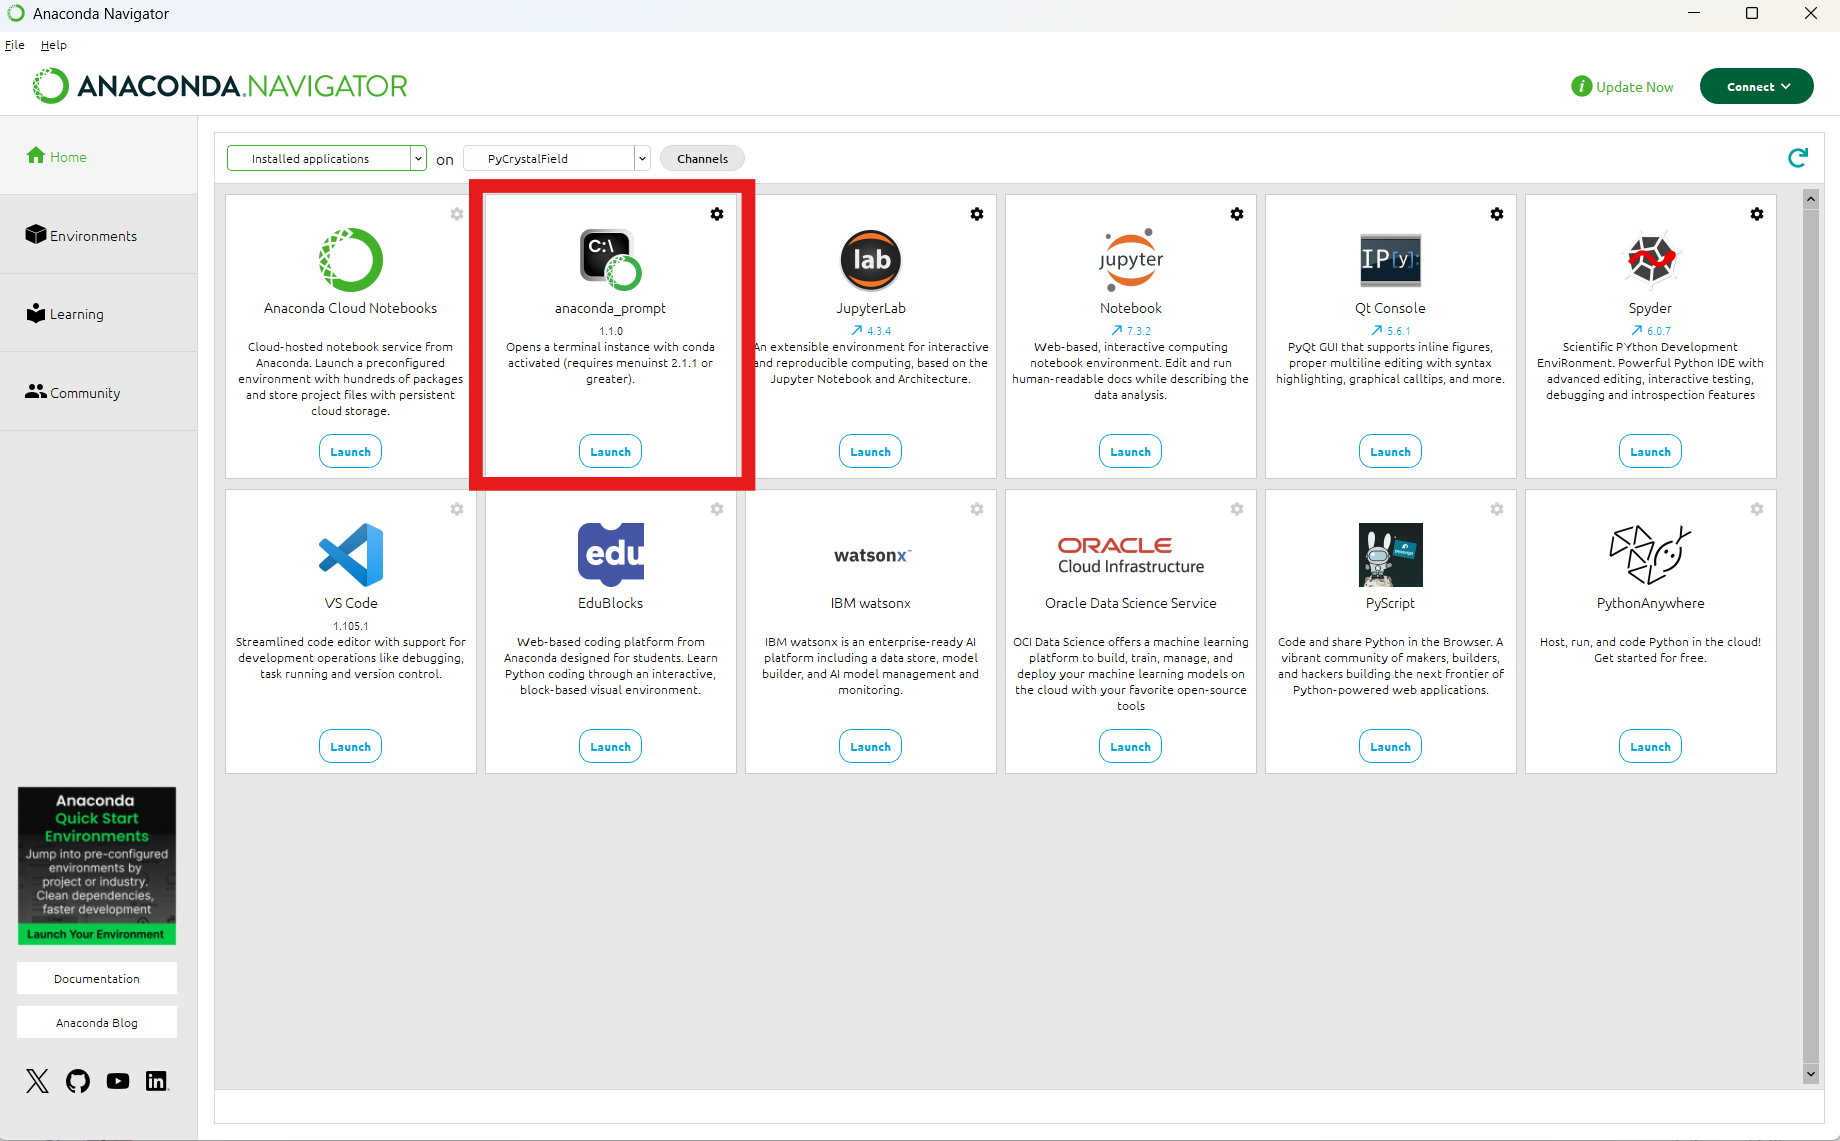
\includegraphics[scale=0.2]{anaconda}
    \end{subfigure}
    \hfill
    \begin{subfigure}{0.45\textwidth}

        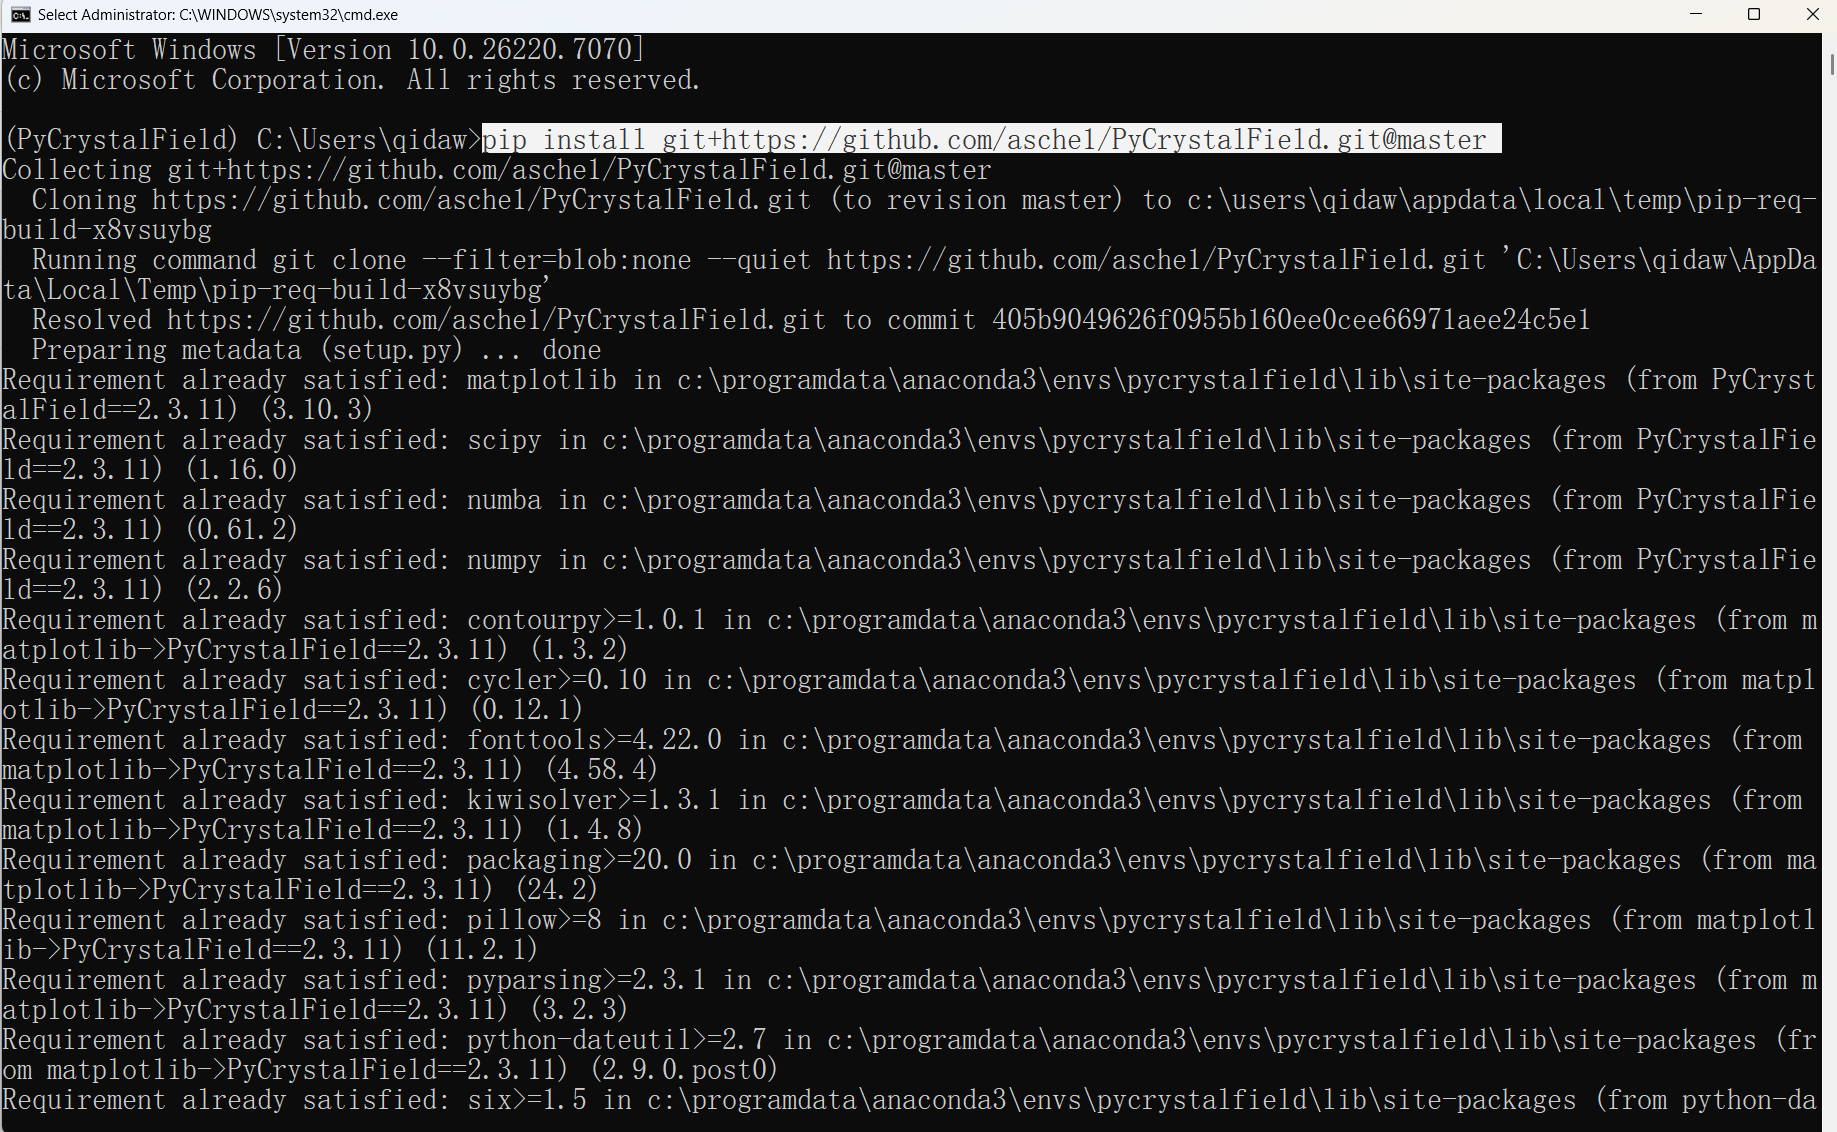
\includegraphics[scale=0.2]{cmd}
    \end{subfigure}
\end{figure}

The program consists of two py files. YZS\_lib.py contains various objects for the program or an individual to access and use. YZS\_fit.py is the main script that is used to perform the fit. We will cover the usage of them in the following sections.

\section{YZS\_lib}

This section only contains methods designed to be used directly by a user.\\

\hrule
\begin{lstlisting}[
    language=Python, 
    showstringspaces=false, 
    breaklines = true,
    stringstyle=\ttfamily,
]
def PCM_Ar(ciffile, mag_ion = None, Zaxis = None, Yaxis = None, 
           crystalImage = False, NumIonNeighbors = 1, ForceImaginary = False, 
           CoordinateNumber = None, MaxDistance = None):
    
    '''Estimates A^n_m<r^n> using the point charge model.

    Options are inherited from the PyCrystalField `importCIF` function.'''
\end{lstlisting}
\hrule
\bigskip
\hrule
\begin{lstlisting}[
    language=Python, 
    showstringspaces=false, 
    breaklines=true,
    stringstyle=\ttfamily
]
def PCM_Eigen(ciffile, mag_ion = None, Zaxis = None, Yaxis = None,
              crystalImage = False, NumIonNeighbors = 1, ForceImaginary = False,
              CoordinateNumber = None, MaxDistance = None, LaTeX = False):
    '''Estimates eigenvalues and eigenvectors using the point charge model.
    
    The LaTeX parameter controls whether the eigenvectors are output in the LaTeX format.'''
\end{lstlisting}
\hrule
\smallskip
{\textbf{Parameters:}} \\
Inherited from PyCrystalField: 
\begin{itemize}
\item ciffile: cif file location
\item mag\_ion: which ion to treat as the central magnetic ion
\item Zaxis: optional, list [a, b, c] defining the desired z axis for the point charge model (using unit cell axes). If None, the axis with the highest rotational symmetry is chosen.
\item Yaxis: optional, list [a, b, c] defining the desired y axis (using unit cell axes). If None, a mirror plane with the normal orthogonal to Zaxis (if one exists) is chosen.
\item crystalImage: optional, boolean, whether to export a sketch of the ligand environment and the defined axes. Default: False.
\item NumIonNeighbors: optional, int, number of nearest neighbor groups to include in the point charge model. If the first six nearest neighbors are all oxygen ions, these are considered as a group. If the next nearest neighbors are two Zn ions, these are considered as a group. etc. Default: 1.
\item ForceImaginary: optional, boolean, force PyCrystalField to include the -m terms in the point charge model (can be useful for comparing two ion sites with different symmetry). Default: False.
\item CoordinationNumber = Number of ions to include in the coordination sphere. If this is specified, it will override whatever is put for NumIonNeighbors. If None, PyCrystalField will guess the number of ions in the coordination sphere.
\item MaxDistance: Maximum allowed distance for included ligands.
\end{itemize}
Native:

\begin{itemize}
\item LaTeX: A bool to determine whether to print results in \LaTeX\ format.
\end{itemize}

\noindent{\textbf{Note:}} 
\begin{enumerate}
\item Point charge model is a \textbf{very} inaccurate model in crystal field theory. \textbf{Never} use this for serious discussions.
\item The oxidation number is determined by \_atom\_site\_type\_symbol (namely, the second column in the loop). PyCrystalField reads the last two characters of this string as the oxidation number. Therefore, you must use a format like "Yb3+" for the program to work correctly.
\item It is recommended to use at most one parameter that determines which ligand to include.
\end{enumerate}

\bigskip
\bigskip
\hrule
\begin{lstlisting}[
    language=Python, 
    showstringspaces=false, 
    breaklines=true,
    stringstyle=\ttfamily
]
def HAM_Eigen(ion, Ardict, LaTeX = False):
    '''Displays the eigenvectors for the ground and excited states of a given Hamiltonian.
    
    ion: string, giving the RE ion to be calculated ("Yb3+", "Ho3+", etc.).
    Ardict: dictionary, giving the CEF parameters Arnm and values. 
    Example: {'Ar20':-0.42, 'Ar40': 0.02, 'Ar44':0.13}.
    The LaTeX parameter controls whether the eigenvectors are output in the LaTeX format.'''
\end{lstlisting}
\hrule
\smallskip
\noindent{\textbf{Parameters:}} 
\begin{itemize}
\item ion: \texttt{`Ce3+', `Pr3+', `Nd3+', `Pm3+', `Sm3+', `Eu3+',`Tb3+', `Dy3+', `Ho3+', `Er3+', `Tm3+', `Yb3+', `U3+', `U4+'}
\item Ardict: A dictionary for term independent crystal parameters, defined as $A_n^m\langle r^n \rangle$
\item LaTeX: Print in the \LaTeX\ or not.
\end{itemize}

\subsection*{Quick Start Guide}
In order to use the library, you must make them accessible in your environment. While there are many ways to do this, if you are only interested in printing information with the above methods, the most straightforward way is to run the YZS\_lib.py file directly in Spyder.

\begin{center}
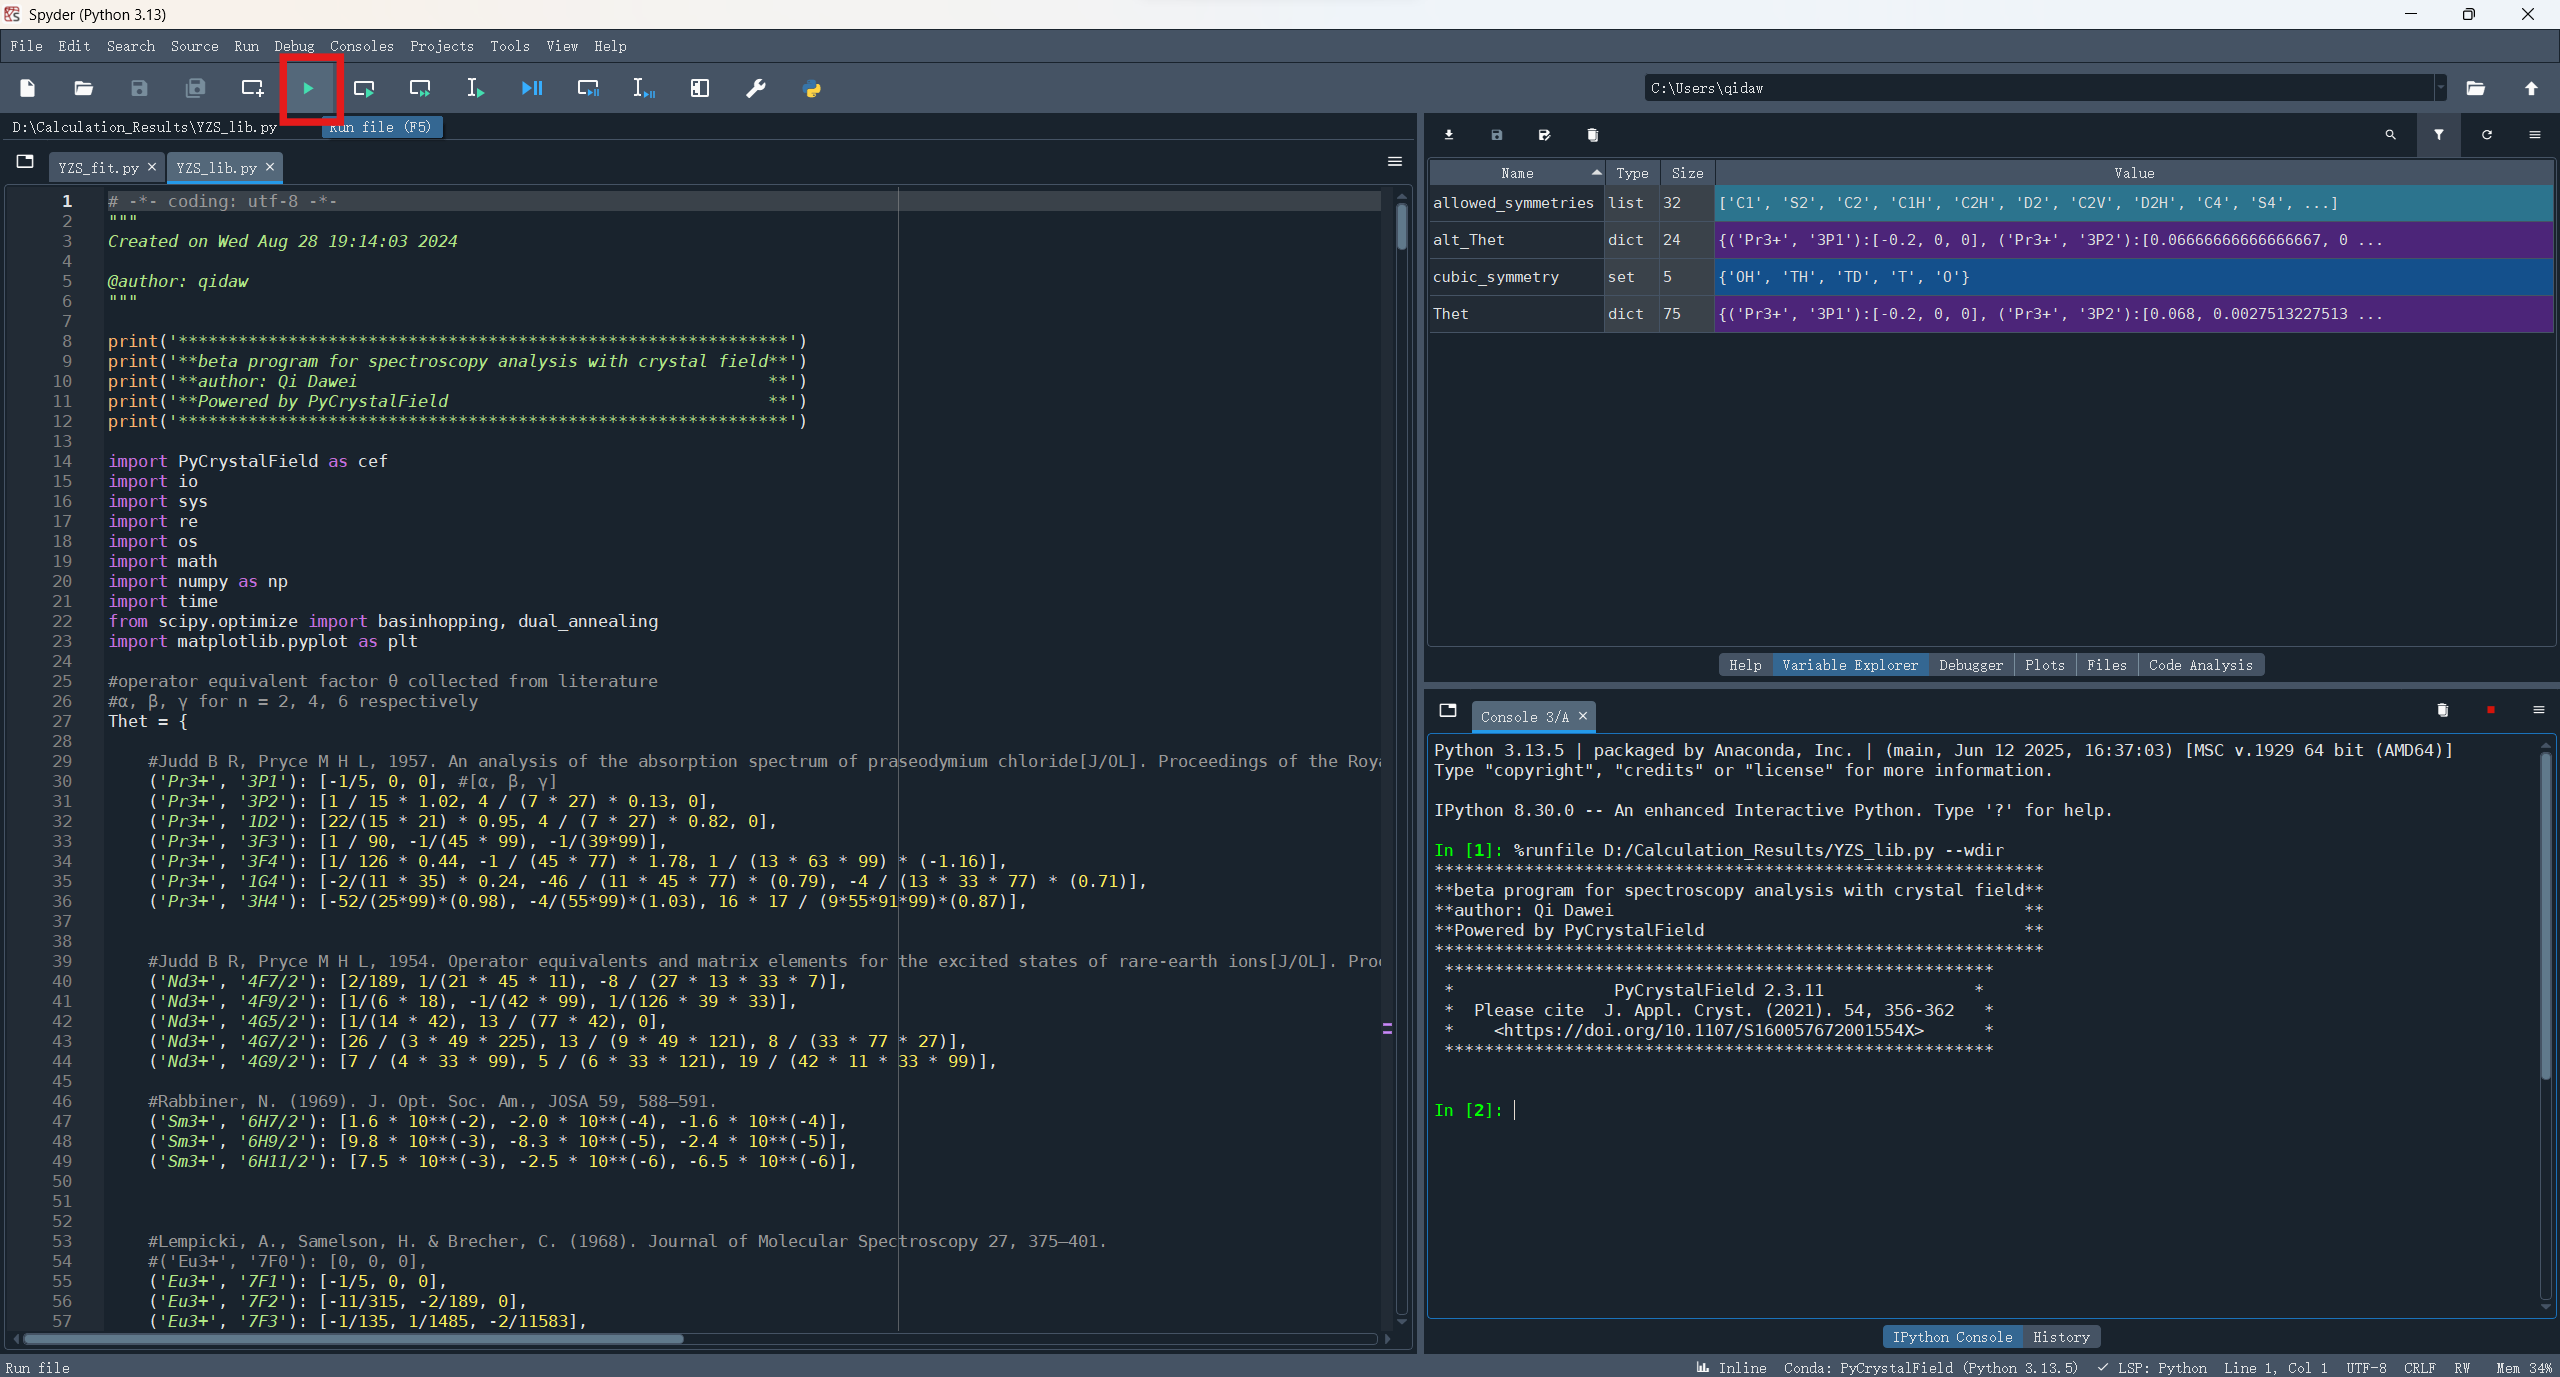
\includegraphics[scale=0.2]{load}
\end{center}

After you have clicked the run button, you will have all the objects of this library in your memory for you to use at your convenience.

For example, for one who wants to get the crystal field parameters $A_n^m\langle r^n \rangle$ for a rare earth ion in a given CIF file, you could do:

\begin{lstlisting}[
    language=Python, 
    showstringspaces=false, 
    breaklines=true,
    stringstyle=\ttfamily
]
PCM_Ar("Yb2Ti2O7.cif")
\end{lstlisting}
in the Spyder console. Then you will get:
\begin{lstlisting}[
    basicstyle=\ttfamily,
    breaklines=True
]
unit cell: 10.01247 10.01247 10.01247 90.0 90.0 90.0
Importing atoms
   104 atoms added
.cif import complete.
No mag_ion ion listed, assuming Yb1 is the central ion.
Central ion: Yb3+ at [0.5, 0.5, 0.5]
    AAAH! There is a super-close atom. Removing it...
 Nearest ligand: O2-
   Identified 8 O2- ligands.
   Found 3 fold axis about [1. 1. 1.]
	Found a near-3-fold axis...  CSM= 1.3750135287169678e-23
   No mirror plane found orthogonal to a rotation axis.
      Found mirror plane at [-0.70710678  0.          0.70710678] 
     Using [0.05766312 0.05766312 0.05766312] as the Z axis and [-0.70710678  0.          0.70710678] as the Y axis.

  Axes for point charge model (in ABC space):
        X axis = [-0.5  1.  -0.5] 
        Y axis = [-1.  0.  1.] 
        Z axis = [1. 1. 1.] 


******************

Estimated A^n_m<r^n> for Yb2Ti2O7.cif:
    A^2_0<r^2>: 16.868941833720378
    A^4_0<r^4>: 25.58835535159091
    A^4_3<r^4>: -193.3041751761479
    A^6_0<r^6>: 2.226809644941047
    A^6_3<r^6>: 20.43874286836878
    A^6_6<r^6>: 21.193714383114003
\end{lstlisting}

\begin{center}
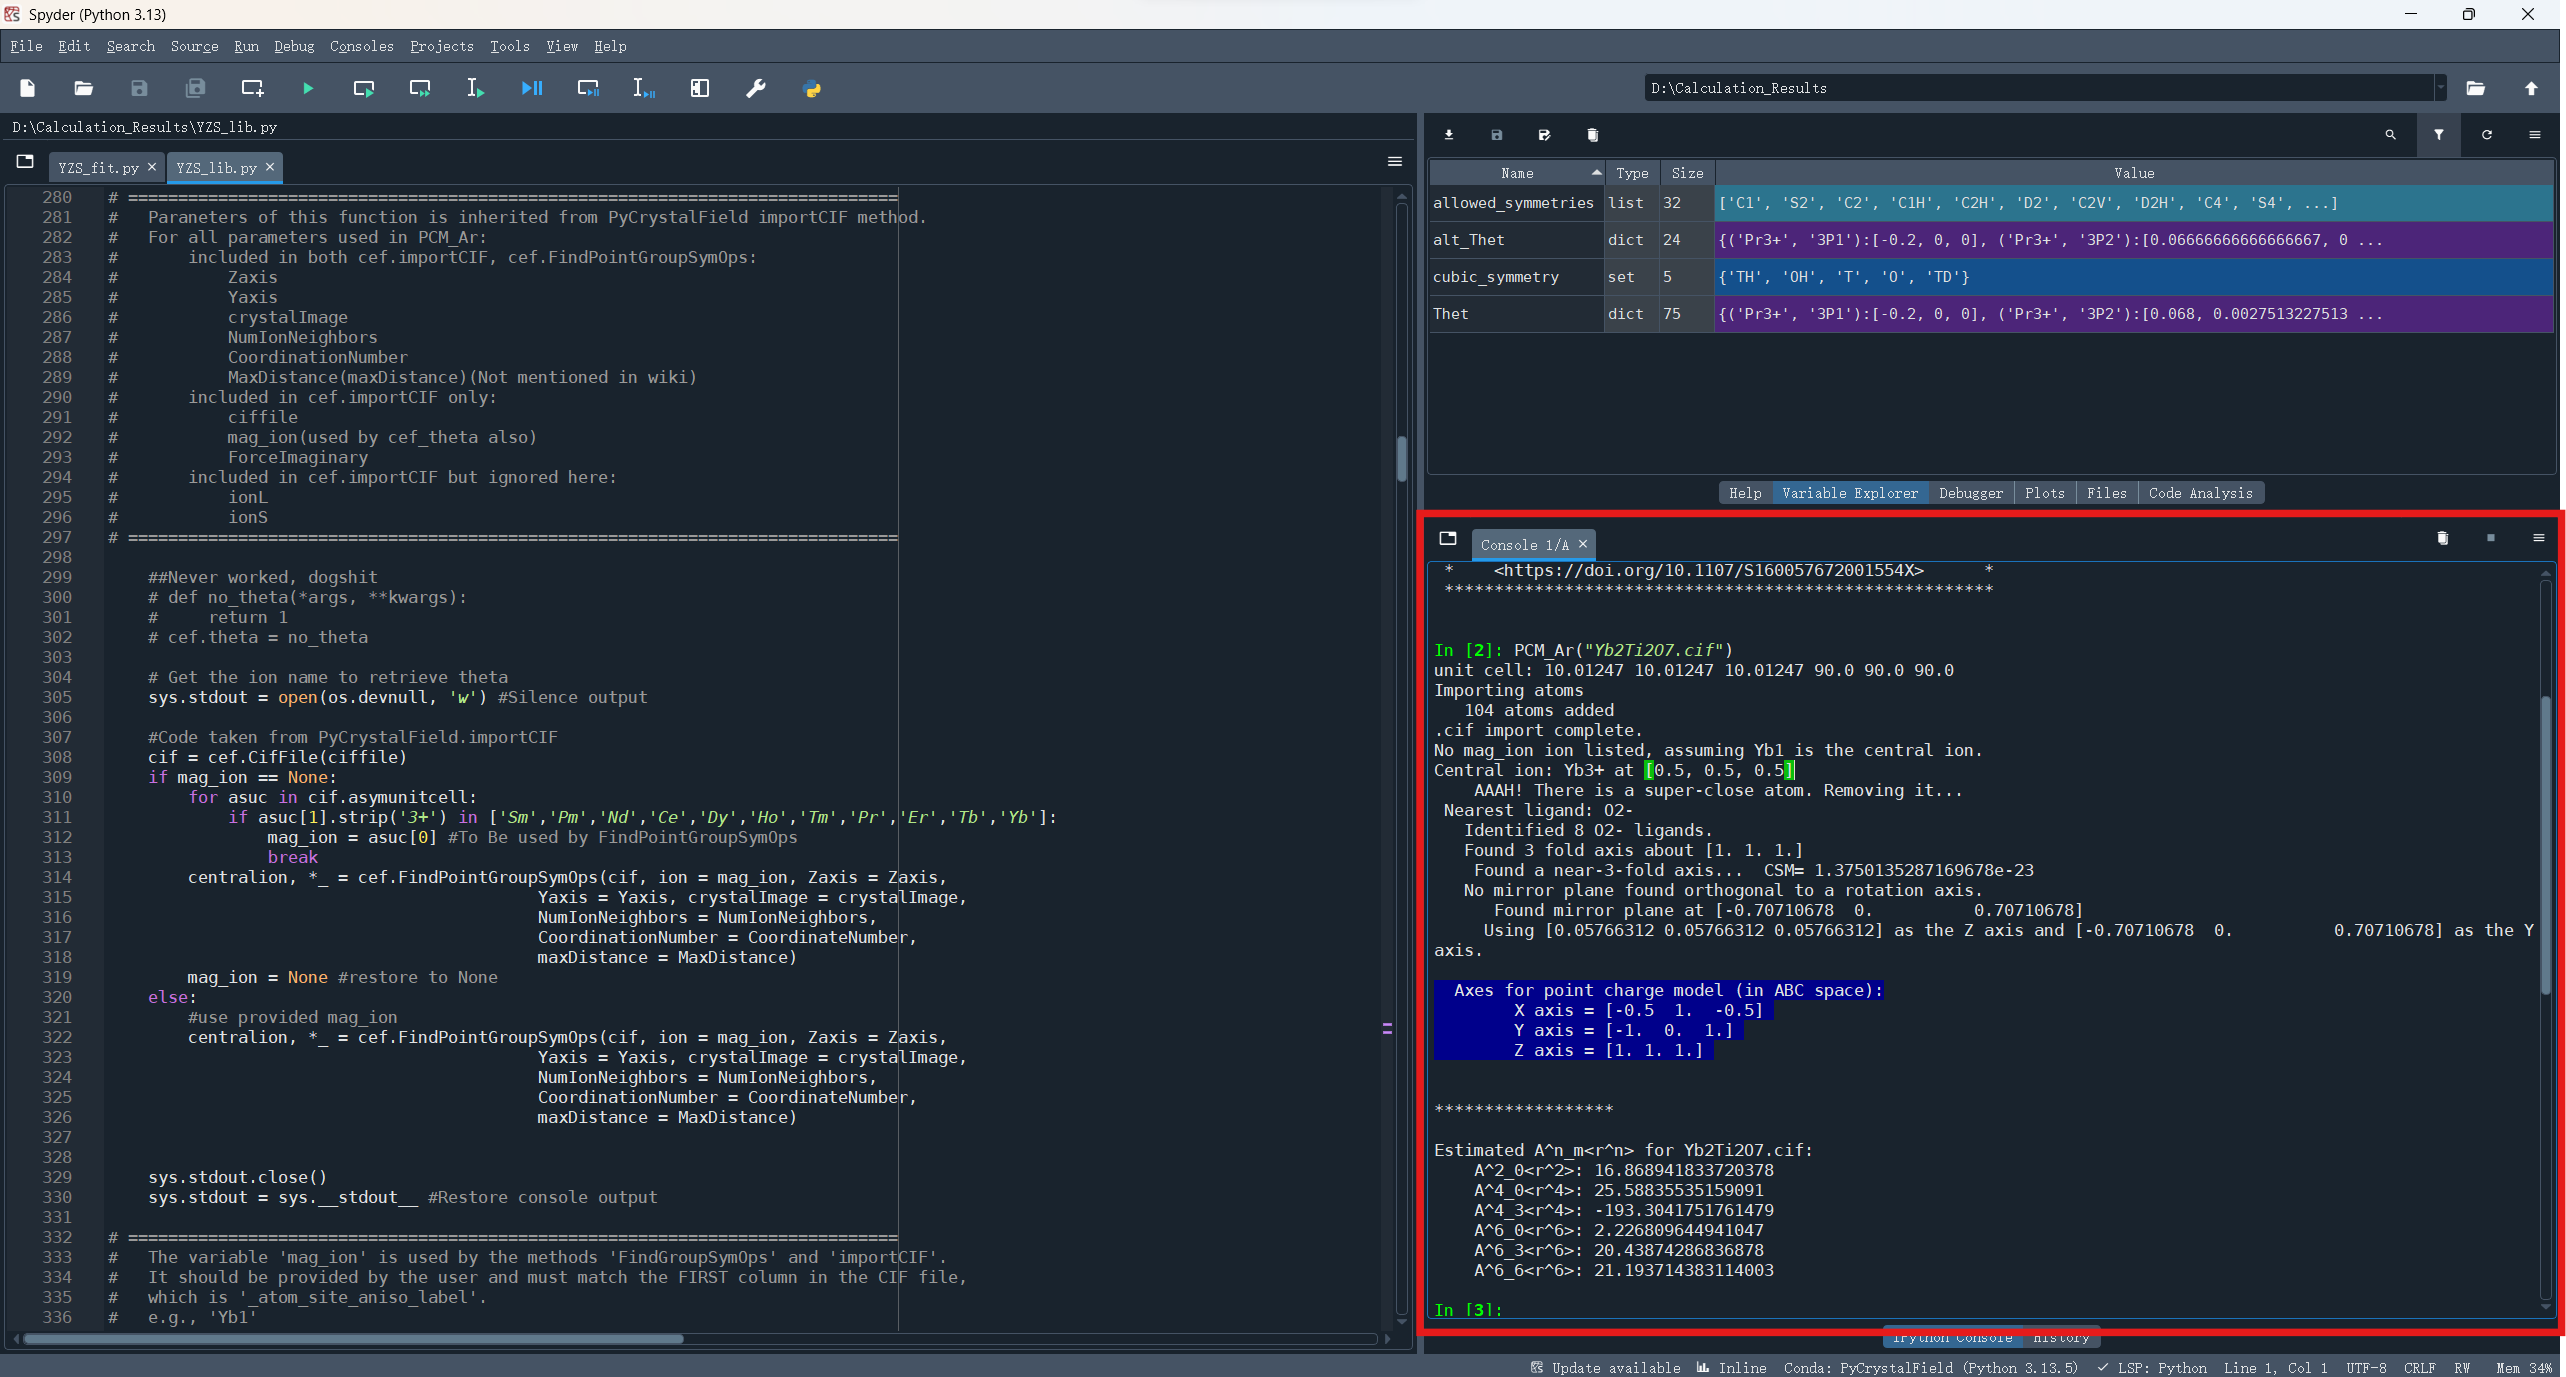
\includegraphics[scale=0.2]{uselib}
\end{center}

You may also check these examples:
\hrule
\smallskip
\noindent{\textbf{Input:}}
\begin{lstlisting}[
    language=Python, 
    showstringspaces=false, 
    breaklines=true,
    stringstyle=\ttfamily,
]
PCM_Eigen("Yb2Ti2O7.cif", LaTeX = True)
\end{lstlisting}
\noindent{\textbf{Output:}}
\begin{lstlisting}[
    basicstyle=\ttfamily,
    breaklines=True
]
unit cell: 10.01247 10.01247 10.01247 90.0 90.0 90.0
Importing atoms
   104 atoms added
.cif import complete.
No mag_ion ion listed, assuming Yb1 is the central ion.
Central ion: Yb3+ at [0.5, 0.5, 0.5]
    AAAH! There is a super-close atom. Removing it...
 Nearest ligand: O2-
   Identified 8 O2- ligands.
   Found 3 fold axis about [1. 1. 1.]
	Found a near-3-fold axis...  CSM= 1.373765767701657e-23
   No mirror plane found orthogonal to a rotation axis.
      Found mirror plane at [-0.70710678  0.          0.70710678] 
     Using [0.05766312 0.05766312 0.05766312] as the Z axis and [-0.70710678  0.          0.70710678] as the Y axis.

  Axes for point charge model (in ABC space):
        X axis = [-0.5  1.  -0.5] 
        Y axis = [-1.  0.  1.] 
        Z axis = [1. 1. 1.] 


******************

Estimated eigenvalue of Yb3+ in Yb2Ti2O7.cif:
 
Multiplet:  2F7/2
\begin{table*}
\caption{Eigenvectors and Eigenvalues...}
\begin{ruledtabular}
\begin{tabular}{c|cccccccc}
E (meV) &$| -\frac{7}{2}\rangle$ & $| -\frac{5}{2}\rangle$ & $| -\frac{3}{2}\rangle$ & $| -\frac{1}{2}\rangle$ & $| \frac{1}{2}\rangle$ & $| \frac{3}{2}\rangle$ & $| \frac{5}{2}\rangle$ & $| \frac{7}{2}\rangle$ \tabularnewline
 \hline 
0.000 & 0.3742 & 0.0 & 0.0 & 0.9214 & 0.0 & 0.0 & -0.1053 & 0.0 \tabularnewline
0.000 & 0.0 & -0.1053 & 0.0 & 0.0 & -0.9214 & 0.0 & 0.0 & 0.3742 \tabularnewline
38.615 & 0.9265 & 0.0 & 0.0 & -0.3764 & 0.0 & 0.0 & -0.0008 & 0.0 \tabularnewline
38.615 & 0.0 & -0.0008 & 0.0 & 0.0 & 0.3764 & 0.0 & 0.0 & 0.9265 \tabularnewline
47.109 & 0.0 & 0.0 & -1.0 & 0.0 & 0.0 & 0.0 & 0.0 & 0.0 \tabularnewline
47.109 & 0.0 & 0.0 & 0.0 & 0.0 & 0.0 & 1.0 & 0.0 & 0.0 \tabularnewline
75.140 & 0.0 & -0.9944 & 0.0 & 0.0 & 0.0972 & 0.0 & 0.0 & -0.0404 \tabularnewline
75.140 & -0.0404 & 0.0 & 0.0 & -0.0972 & 0.0 & 0.0 & -0.9944 & 0.0 \tabularnewline
\end{tabular}\end{ruledtabular}
\label{flo:Eigenvectors}
\end{table*}
 
Multiplet:  2F5/2
\begin{table*}
\caption{Eigenvectors and Eigenvalues...}
\begin{ruledtabular}
\begin{tabular}{c|cccccc}
E (meV) &$| -\frac{5}{2}\rangle$ & $| -\frac{3}{2}\rangle$ & $| -\frac{1}{2}\rangle$ & $| \frac{1}{2}\rangle$ & $| \frac{3}{2}\rangle$ & $| \frac{5}{2}\rangle$ \tabularnewline
 \hline 
0.000 & 0.0 & 0.0 & -0.9377 & 0.0 & 0.0 & 0.3475 \tabularnewline
0.000 & -0.3475 & 0.0 & 0.0 & -0.9377 & 0.0 & 0.0 \tabularnewline
35.730 & -0.9377 & 0.0 & 0.0 & 0.3475 & 0.0 & 0.0 \tabularnewline
35.730 & 0.0 & 0.0 & -0.3475 & 0.0 & 0.0 & -0.9377 \tabularnewline
58.839 & 0.0 & -1.0 & 0.0 & 0.0 & 0.0 & 0.0 \tabularnewline
58.839 & 0.0 & 0.0 & 0.0 & 0.0 & -1.0 & 0.0 \tabularnewline
\end{tabular}\end{ruledtabular}
\label{flo:Eigenvectors}
\end{table*}
\end{lstlisting}
\hrule
\bigskip
\hrule
\smallskip
\noindent{\textbf{Input:}}
\begin{lstlisting}[
    language=Python, 
    showstringspaces=false, 
    breaklines=true,
    stringstyle=\ttfamily
]
HAM_Eigen(ion='Yb3+', Ardict={'Ar20': 16.868941833720378, 'Ar40': 25.58835535159091, 'Ar43': -193.3041751761479, 'Ar60': 2.226809644941047, 'Ar63': 20.43874286836878, 'Ar66': 21.193714383114003})
\end{lstlisting}
\noindent{\textbf{Output:}}
\begin{lstlisting}[
    basicstyle=\ttfamily,
    breaklines=True
]
Ion:  Yb3+
Multiplet:  2F7/2
{'B20': 0.53552196297525, 'B40': -0.04430884043565526, 'B43': 0.3347258444608622, 'B60': 0.000329568157019432, 'B63': 0.003024936969455549, 'B66': 0.0031366728653737376}

 Eigenvalues 	 Eigenvectors
		---------------------------------------------------------------
0.00000 	|  [ 0.374  0.     0.     0.921  0.     0.    -0.105  0.   ]  |
0.00000 	|  [ 0.    -0.105  0.     0.    -0.921  0.     0.     0.374]  |
38.61543 	|  [ 0.926  0.     0.    -0.376  0.     0.    -0.001  0.   ]  |
38.61543 	|  [ 0.    -0.001  0.     0.     0.376  0.     0.     0.926]  |
47.10950 	|  [ 0.  0. -1.  0.  0.  0.  0.  0.]  |
47.10950 	|  [0. 0. 0. 0. 0. 1. 0. 0.]  |
75.14028 	|  [ 0.    -0.994  0.     0.     0.097  0.     0.    -0.04 ]  |
75.14028 	|  [-0.04   0.     0.    -0.097  0.     0.    -0.994  0.   ]  |
		---------------------------------------------------------------

Ion:  Yb3+
Multiplet:  2F5/2
{'B20': 0.9639395333554501, 'B40': -0.16246574826406926, 'B43': 1.2273280963564948, 'B60': 0.0, 'B63': 0.0, 'B66': 0.0}

 Eigenvalues 	 Eigenvectors
		-------------------------------------------------
0.00000 	|  [-0.348  0.     0.    -0.938  0.     0.   ]  |
0.00000 	|  [ 0.     0.    -0.938  0.     0.     0.348]  |
35.72994 	|  [-0.938  0.     0.     0.348  0.     0.   ]  |
35.72994 	|  [ 0.     0.    -0.348  0.     0.    -0.938]  |
58.83890 	|  [ 0. -1.  0.  0.  0.  0.]  |
58.83890 	|  [ 0.  0.  0.  0. -1.  0.]  |
		-------------------------------------------------
\end{lstlisting}
\hrule
\smallskip
\noindent{\textbf{Note:}}
\begin{itemize}
\item The first occurrence of ``AAAH ! There is a super - close atom . Removing it ..." is a bug from PyCrystalField
\item For new Python users: when specifying a parameter in a function call, always use the \texttt{parameter = something} pattern. Separate each argument with a comma, and simply ignore any parameters you don't want to change.
\end{itemize}

\section{YZS\_fit}
Here comes our big story: fitting the crystal field Hamiltonian to optical spectroscopy to reproduce experimental energy levels.

All the information for fitting, including settings and experimental data is included in a plain text file. You are going to specify the path of your text file in the file\_path then run the entire YZS\_fit.

\begin{center}
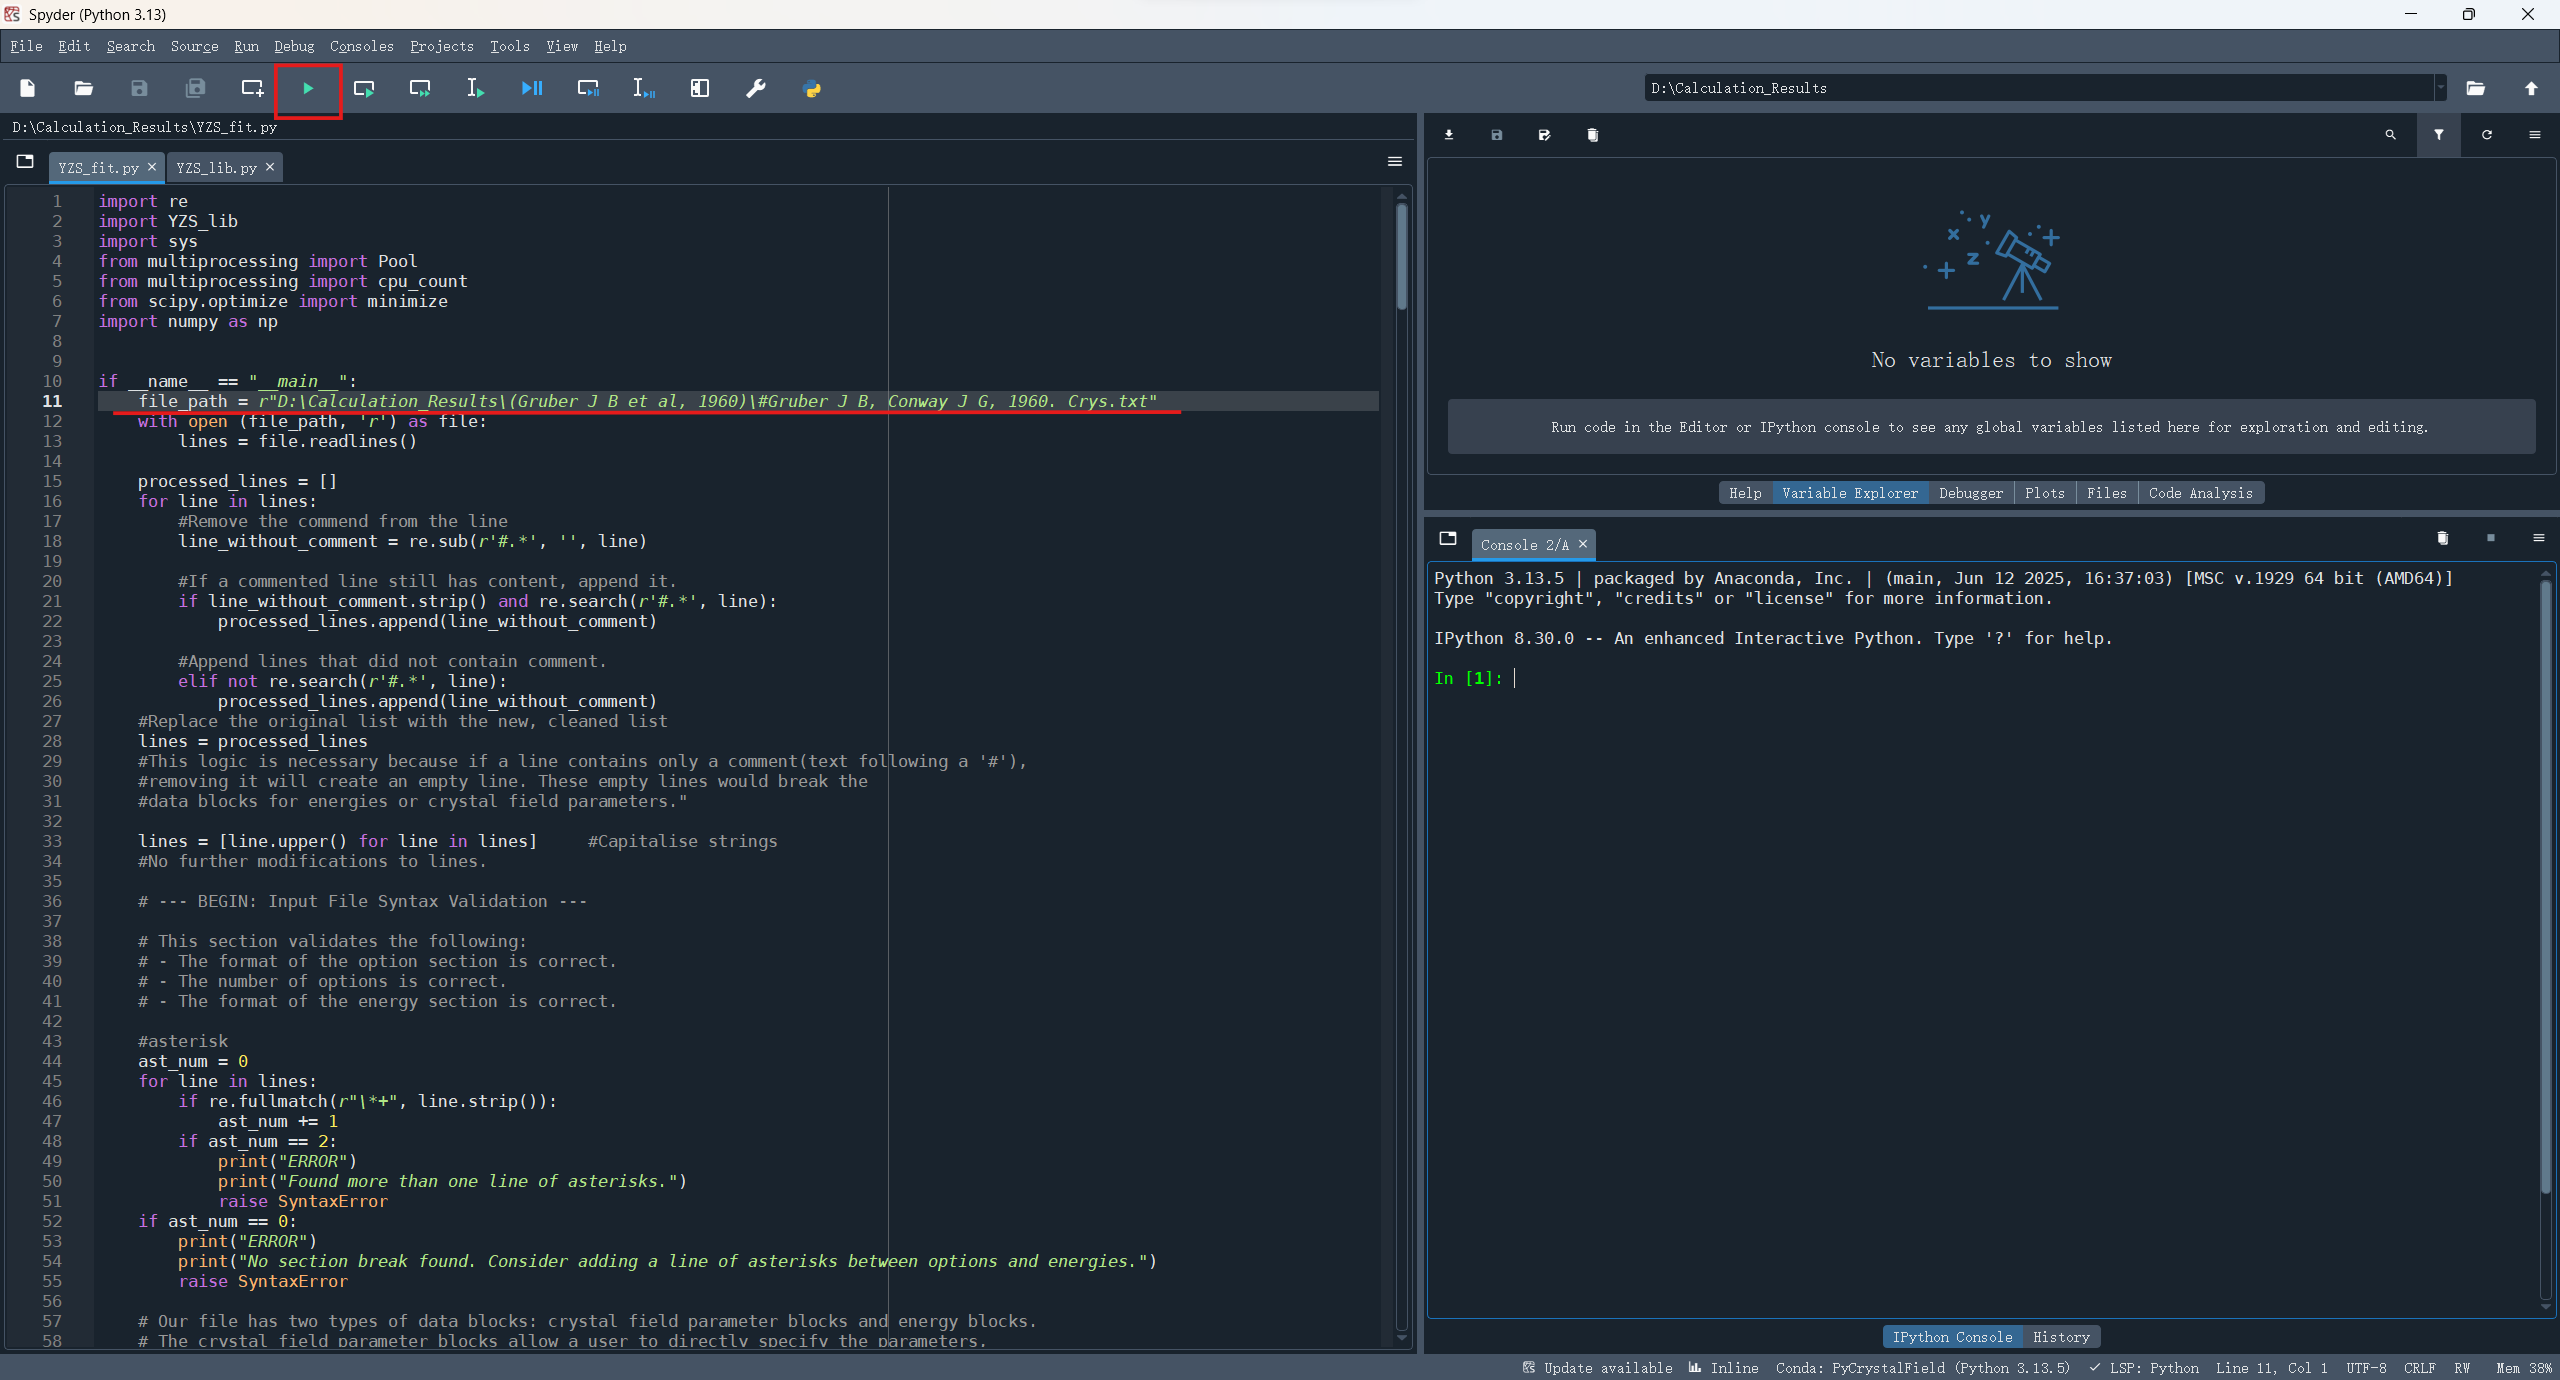
\includegraphics[scale=0.2]{usefit}
\end{center}

We are going to talk about the format of the text file. Make sure you are reading it when comparing it with the given templates.

The text file is split into two parts: the first part for configurations, the second part for experimental data. The two parts are separated by a line of asterisks. The file itself is case-insensitive.

Comments are allowed in the text file. All content after a \# is ignored.

\noindent \textbf{Configurations}

The configuration part of the file follows a keyword-value pattern, where you specify the keyword first, followed by some spaces and the value. No indentation is allowed before the keyword.

\noindent Mandatory keywords include:
\begin{enumerate}
\item \texttt{ION}    name of the magnetic ion like `Er3+'
\item \texttt{SYMMETRY}    site symmetry of the magnetic ion
\item \texttt{PARAMETERS}    allowed crystal field parameters
\end{enumerate}
Optional keywords:
\begin{enumerate}
\item \texttt{BOUNDS}    global bound for the crystal field parameters
\item \texttt{MCTIME}    calculation time for the monte carlo search
\item \texttt{alt\_Thet}    True or False, determines whether to use the alternative theta values.
\end{enumerate}
Please check the template for their usage. Please notice that the PARAMETERS keyword is a little bit different. It is followed by a block from the next line. All lines in the block must start with a mandatory four-space indentation. The block is broken by the first line that does not follow this rule. You are allowed to specify a specific bound for the parameter, but you are also allowed to leave it.

Also notice that SYMMETRY and PARAMETERS are not allowed to be specified simultaneously. In fact, we are using the site symmetry to determine which crystal field parameters are allowed to appear.

When you specify the global bound and the individual bound simultaneously, the individual bound on the specific parameter will prevail.

\noindent \textbf{Energies}\\
You should first specify the term symbol, then starting from the next line listing experimental energies from that spectral term. If some of the expected values are not available from experiment, just type \texttt{None} for each such level instead.

A blank line is required to separate different term symbol blocks. No indentation is ever allowed on any lines in the energies section.

A user should have the energies of each spectral term sorted in the ascending order.



\lstset{
  basicstyle=\ttfamily, % Set font to a monospaced family
  breaklines=true,      % Enable automatic line breaking
  postbreak=\mbox{\textcolor{gray}{$\hookrightarrow$}\space}  
}

\subsection*{template\_sym}
\begin{lstlisting}
# Case insensitive
# Energy unit: meV

#BRECHER C, SAMELSON H, LEMPICKI A, et al, 1967. Polarized Spectra and Crystal-Field Parameters of Eu+3 in YVO4[J/OL]. Physical Review, 155(2): 178-187. DOI:10.1103/PhysRev.155.178.


# mandatory
ION   EU3+
SYMMETRY D2d

#optional
TIME    5  # minutes
BOUNDS    (-200, 200)
alt_Thet  False
 

***************************************************************************************

7F1
41.3731271
46.5680148

7F2
122.17284819999999
138.3774263
116.0976812
128.7811421

7F3
232.220159
235.939649
229.9636684
242.634731
236.06363199999998

7F4
379.759929
356.947057
362.402309
334.7541
355.54604909999995
370.5107972
350.87189

7F5
471.1354
464.93625
479.81421
503.99089499999997
485.393445
489.608867
487.005224
479.81421


\end{lstlisting}
\hrule
\subsection*{template\_asym}
\begin{lstlisting}
# Case insensitive
# Energy unit: meV

#BRECHER C, SAMELSON H, LEMPICKI A, et al, 1967. Polarized Spectra and Crystal-Field Parameters of Eu+3 in YVO4[J/OL]. Physical Review, 155(2): 178-187. DOI:10.1103/PhysRev.155.178.

ION    Eu3+

#Do not specify symmetry in this case.
PARAMETERS 
    Ar20    (-10, 10)    #bounds could be ignored
    Ar40    (-10, 10)
    Ar60    (-10, 10)
    Ar44    (-100, 100)
    Ar64    (-10, 10)

#optional
TIME   5 # minutes
BOUNDS    (-200, 200)

***************************************************************************************

7F1
41.3731271
46.5680148

7F2
122.17284819999999
138.3774263
116.0976812
128.7811421

7F3
232.220159
235.939649
229.9636684
242.634731
236.06363199999998

7F4
379.759929
356.947057
362.402309
334.7541
355.54604909999995
370.5107972
350.87189

7F5
471.1354
464.93625
479.81421
503.99089499999997
485.393445
489.608867
487.005224
479.81421

\end{lstlisting}
\hrule
\subsection*{template\_misen}
\begin{lstlisting}
# Case insensitive
# Energy unit: meV

#BRECHER C, SAMELSON H, LEMPICKI A, et al, 1967. Polarized Spectra and Crystal-Field Parameters of Eu+3 in YVO4[J/OL]. Physical Review, 155(2): 178-187. DOI:10.1103/PhysRev.155.178.

ION    EU3+

#Do not specify symmetry in this case.
PARAMETERS 
    Ar20    (-10, 10)    #bounds could be ignored
    Ar40    (-10, 10)
    Ar60    (-10, 10)
    Ar44    (-100, 100)
    Ar64    (-10, 10)

#optional
MCTIME    5    # minutes

***************************************************************************************

7F1
41.3731271
46.5680148

7F2
122.17284819999999
138.3774263
116.0976812
128.7811421

7F3
232.220159
235.939649
229.9636684
242.634731
236.06363199999998

7F4
379.759929
356.947057
362.402309
334.7541
355.54604909999995
370.5107972
350.87189

7F5
464.93625
471.1354
None
479.81421
485.393445
487.005224
None
503.99089499999997

\end{lstlisting}
\subsection*{Output:}
\begin{lstlisting}
*************************************************************
**beta program for spectroscopy analysis with crystal field**
**author: Qi Dawei                                         **
**Powered by PyCrystalField                                **
*************************************************************
Warning: The energy list for term '7F2' was not sorted.
Warning: The energy list for term '7F3' was not sorted.
Warning: The energy list for term '7F4' was not sorted.
Warning: The energy list for term '7F5' was not sorted.
The following term symbols will be fitted:
['7F1', '7F2', '7F3', '7F4', '7F5']
Ion: EU3+
Energy unit: mev
 
==================================================================
*************************Resuls***********************************
 
Fitted Crystal Field Parameters:
Ar20: 1.2009628152103415
Ar40: 5.975048118891678
Ar44: -78.44205875107434
Ar60: 9.330760830276876
Ar64: 8.092483186080663
 
Sum of Squared Differences: 261.4862693451755
 
Comparison between theoretical and experimental energies: 
Theoretical      Experimental
7F1
  0.000000  :    0.000000
  0.720578  :    5.194888
 
7F2
  0.000000  :    0.000000
  6.670476  :    6.075167
 14.132023  :   12.683461
 19.921793  :   22.279745
 
7F3
  0.000000  :    0.000000
  2.770734  :    2.256491
  7.046267  :    5.975981
  8.103428  :    6.099964
 12.742247  :   12.671063
 
7F4
  0.000000  :    0.000000
  7.729734  :   16.117790
 22.855705  :   20.791949
 24.694282  :   22.192957
 25.318587  :   27.648209
 26.539388  :   35.756697
 42.365663  :   45.005829
 
7F5
  0.000000  :    0.000000
  3.381350  :    6.199150
 10.665387  :   14.877960
 13.946879  :   14.877960
 21.685638  :   20.457195
 24.703529  :   22.068974
 27.598818  :   24.672617
 36.558972  :   39.054645
\end{lstlisting}
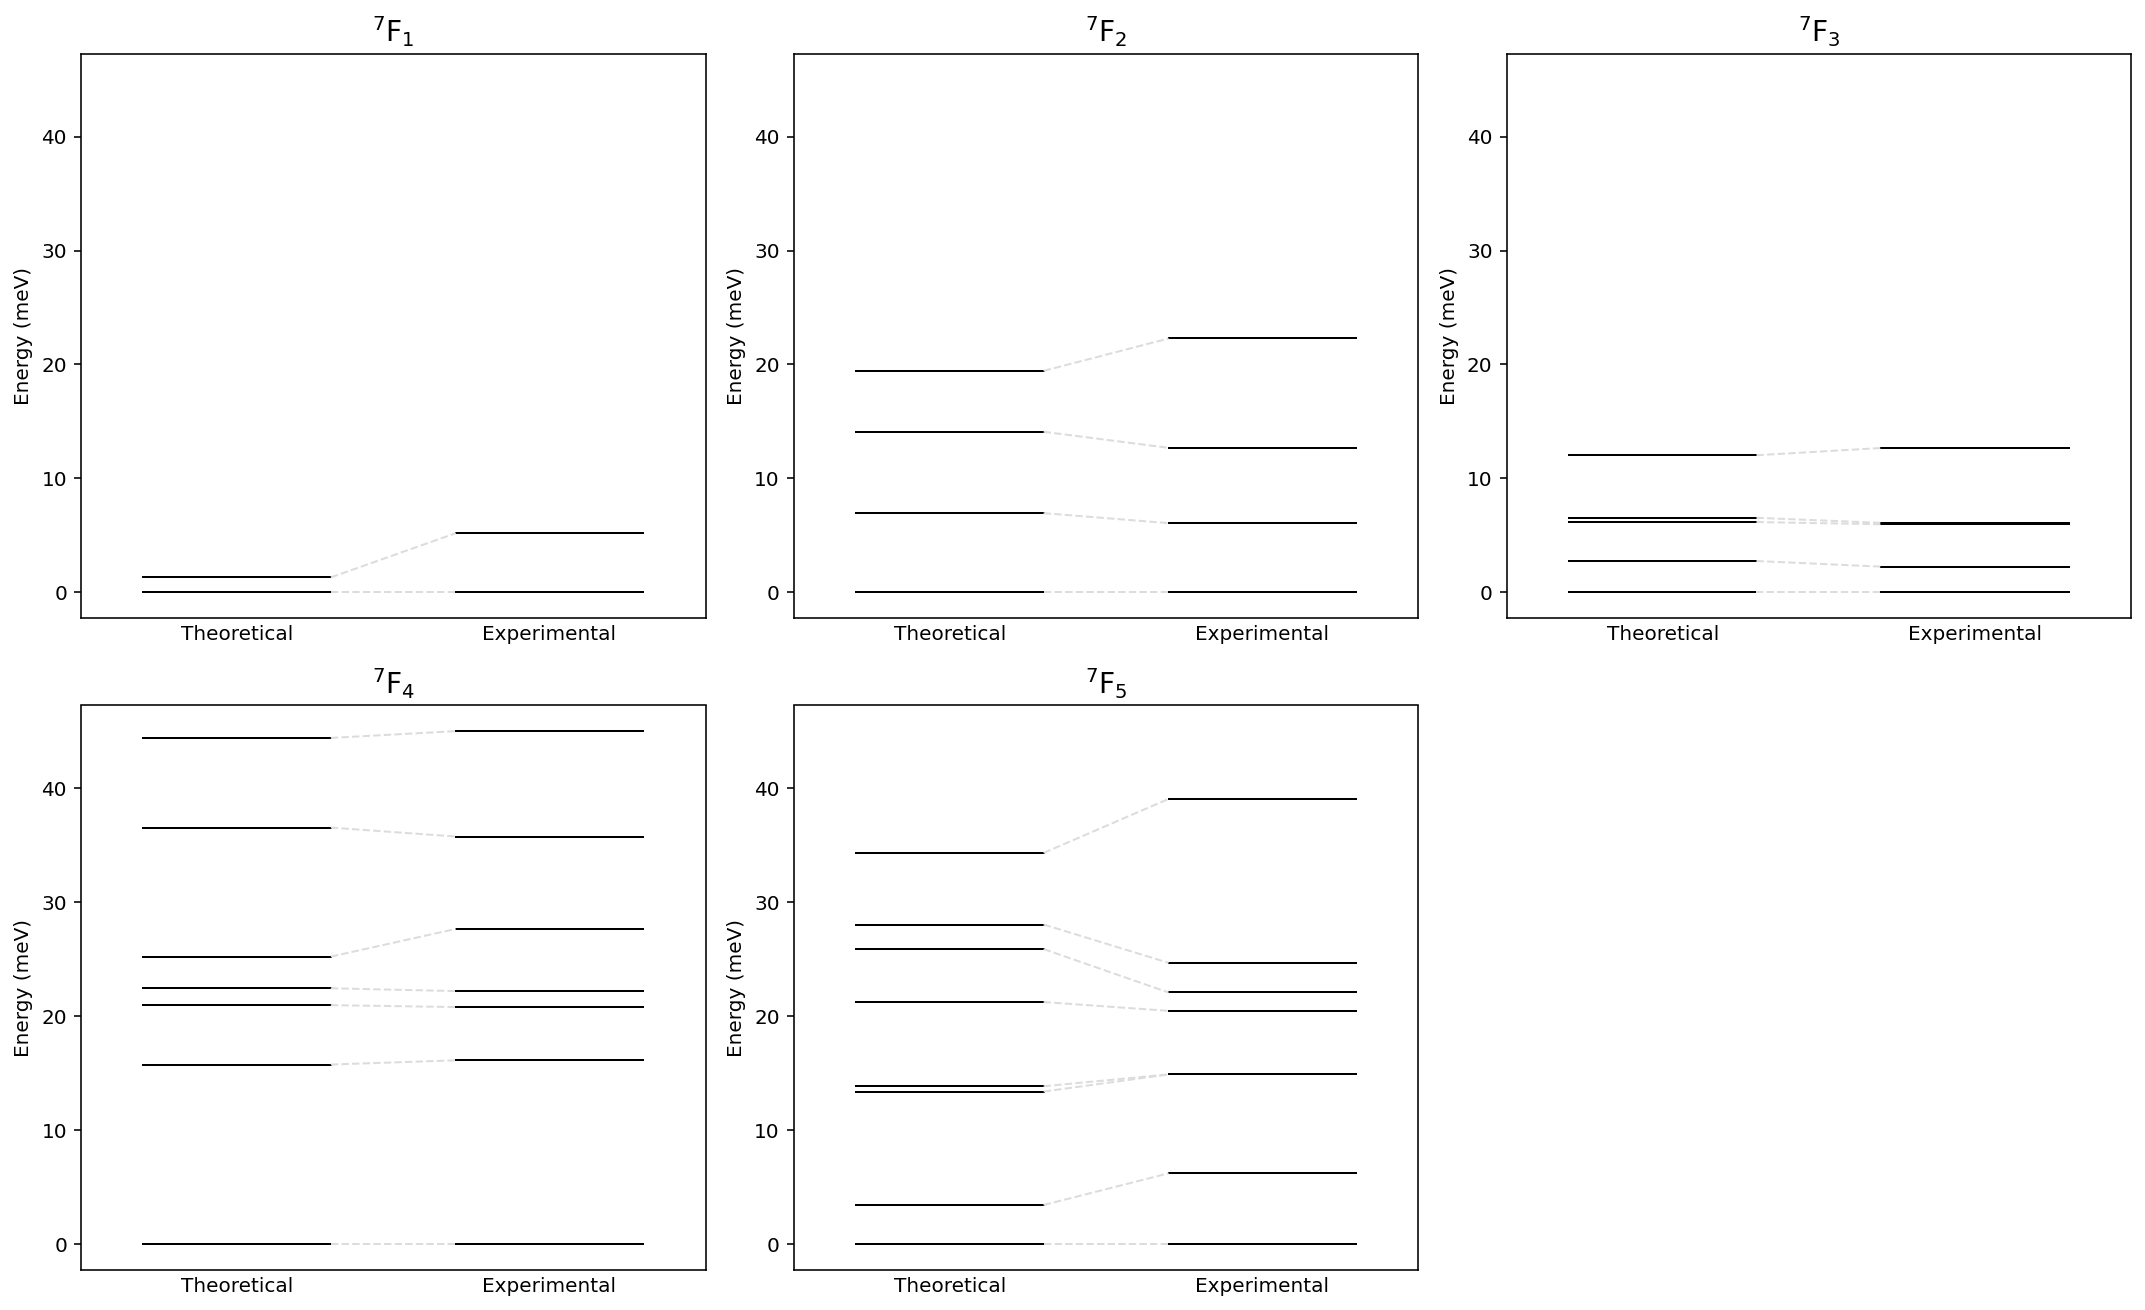
\includegraphics[scale=0.4]{res}

\appendix

\section{Theory}
We assume that the 4f electrons of a rare earth ion located in a crystal are subjected to an external potential field applied by the outer ligands. The field satisfies the Laplace equation
$$\nabla^2V(r, \theta, \phi)=0$$
where V can be expanded as 
$$ V =\sum _{\ell =0}^{\infty }\sum _{m=-\ell }^{\ell }A_{\ell, m}Y_{\ell }^{m}(r, \theta ,\varphi)$$
This develops into the crystal field Hamiltonian (Stevens equivalent operator method \cite{stevensMatrixElementsOperator1952}):
$$\mathscr{H}=\sum_{nm}[(A_n^m\langle r^n \rangle )\theta_n]O_n^m$$
$O_n^m$ are angular momentum operators called Stevens Operator, and $\theta$ is a scaling factor. The $A_n^m\langle r^n \rangle$, often called the Crystal Field Parameters, represent the effect of the ligand environment on the central ion. Their values are often obtained from fitting.

Since the crystal field strength for rare earth ions is relatively small compared to other interactions, such as spin-orbit coupling, we treat this Hamiltonian as a perturbation on the effective J states.

As recommended by many, I found that the all-time classic paper \cite{hutchingsPointChargeCalculationsEnergy1964} is one of the best resources for one to understand Crystal Field Theory.




\bibliographystyle{alpha}
\bibliography{guide} 

\end{document}